\section{Results and Discussion}

\subsection{Comparing Aggregate Statistics of Community Structure}

We begin by examining the overall statistics for the communities inferred by OSLOM using the weightings defined in the previous sections. The number of communities by community type is given in Table~\ref{Table-comm_count}. We see that the topic- and interaction-based networks admit the most communities. The activity-based network admits the fewest communities.  One advantage of the OSLOM over many other community detection algorithms is that it explicitly accounts for singleton `communities': those nodes who do not belong to \emph{any} extant communities. This is especially important when a network is collected via a breadth-first search, as in our network, where we begin from a seed node and then branch out. Such a search, once terminated, will result in a collection of nodes on the periphery of the network that may not belong to any community in the core.

% See here
% 	http://arxiv.org/pdf/1202.2684v2.pdf
% for possible useful references on core-periphery networks.

We see in Table~\ref{Table-comm_count} that the topic- and interaction-based communities have the most singletons, with the activity-based community dominating this measure. This result for the activity-based community is partially an artifact of a property of the retweet/mention weighting: 717 of the users were disconnected from the network by how the weights were defined, resulting in `orphan' nodes which we have included in the collection of singletons for all of our analyses. However, even after accounting for this artifact, the interaction-based network still has the most non-orphan singletons. This seems to indicate that a large fraction of the 6917 (nearly 25\%) do not interact with each other in a concerted way that would mark them as a community under our interaction-based definition. This agrees with a result previously reported in~\cite{romero2011influence} about how most users passively interact with incoming information on Twitter.

\begin{table}[ht]
	\caption{Number of non-singleton communities and singletons by community type: S(tructural), A(ctivity-based), T(opic-based), and I(nteraction-based).}
	\centering
	\begin{tabular}{| c | c | c |}
		\hline Community Type & \# of Communities & \# of Singletons \\ \hline
		% Structural & 201 \\
		% Activity, Lag 1 & 101 \\
		% Activity, Lag 2 & 99 \\
		% Activity, Lag 3 & 106 \\
		% Activity, Lag 4 & 105 \\
		% Activity, Lag 5 & 107 \\
		% Activity, Lag 6 & 106 \\
		% Topic & 289 \\
		% Interaction & 252 \\ \hline
		S & 201 & 308 \\
		A, Lag 1 & 101 & 951 \\
		A, Lag 2 & 99 & 600 \\
		A, Lag 3 & 106 & 611 \\
		A, Lag 4 & 105 & 668 \\
		A, Lag 5 & 107 & 632 \\
		A, Lag 6 & 106 & 642 \\
		T & 289 & 1064 \\
		I & 252 & 2436 (1719) \\ \hline
	\end{tabular}
	\label{Table-comm_count}
\end{table}

Next we consider the distribution of community sizes across the community types. The complementary cumulative distribution of community sizes is given in Figure~\ref{Fig-community_size_distribution}. Note that both axes are plotted on log-scales. Thus, for a fixed community size $s$, Figure~\ref{Fig-community_size_distribution} shows the proportion of communities of size greater than $s$ for each community type. We see that the community distributions have longer tails for the non-structural networks, and that the interaction-based network has the longest tail. The largest communities for the structural, activity-based, topic-based, and interaction-based networks have 198, 358, 338, and 811 members, respectively. Most importantly, we see that the distributions of community sizes differ across the community types, highlighting that the different networks give rise to different large-scale community structure dependent on the particular weighting of the structural network.

\begin{figure}[ht]
  \centering
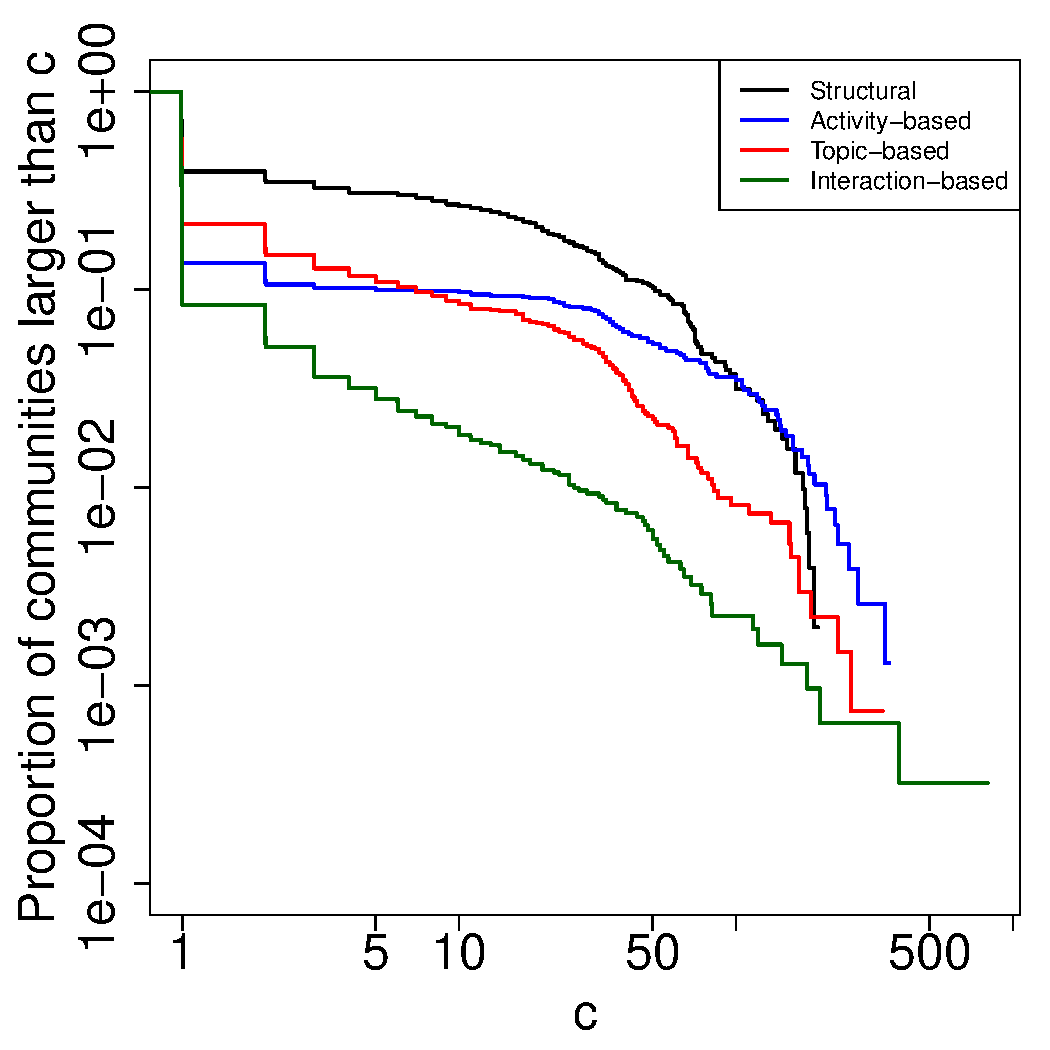
\includegraphics[width=0.50\textwidth]{comm_sizes_ecdf_loglog.pdf}
\caption{The proportion of communities greater than $s$ in size, across the different community types. Note the logarithmic scale on the horizontal and vertical axes.}
\label{Fig-community_size_distribution}
\end{figure}

% Next, we compare the number of users which belong to more than one community. Figure~\ref{Fig-overlap_plot} shows the number of users belonging to 2, 3, or 4 communities. We see that as the number of mixed membership communities increases, the number of users with that number of mixed memberships decreases. This is especially true for the activity-based community \textbf{TK: speculate on what this means? Or save for the results section?}.  In addition, \textbf{TK: mention the 5, 6, and 7 cases, not included in the figure}. This corresponded to \textbf{TK: investigate which users are the high-overlap and what communities they belong to.}

% % The user with a structural overlap of 7 communities was 1630261,
% %	https://twitter.com/marksilva

% \begin{figure}[ht]
%   \centering
% 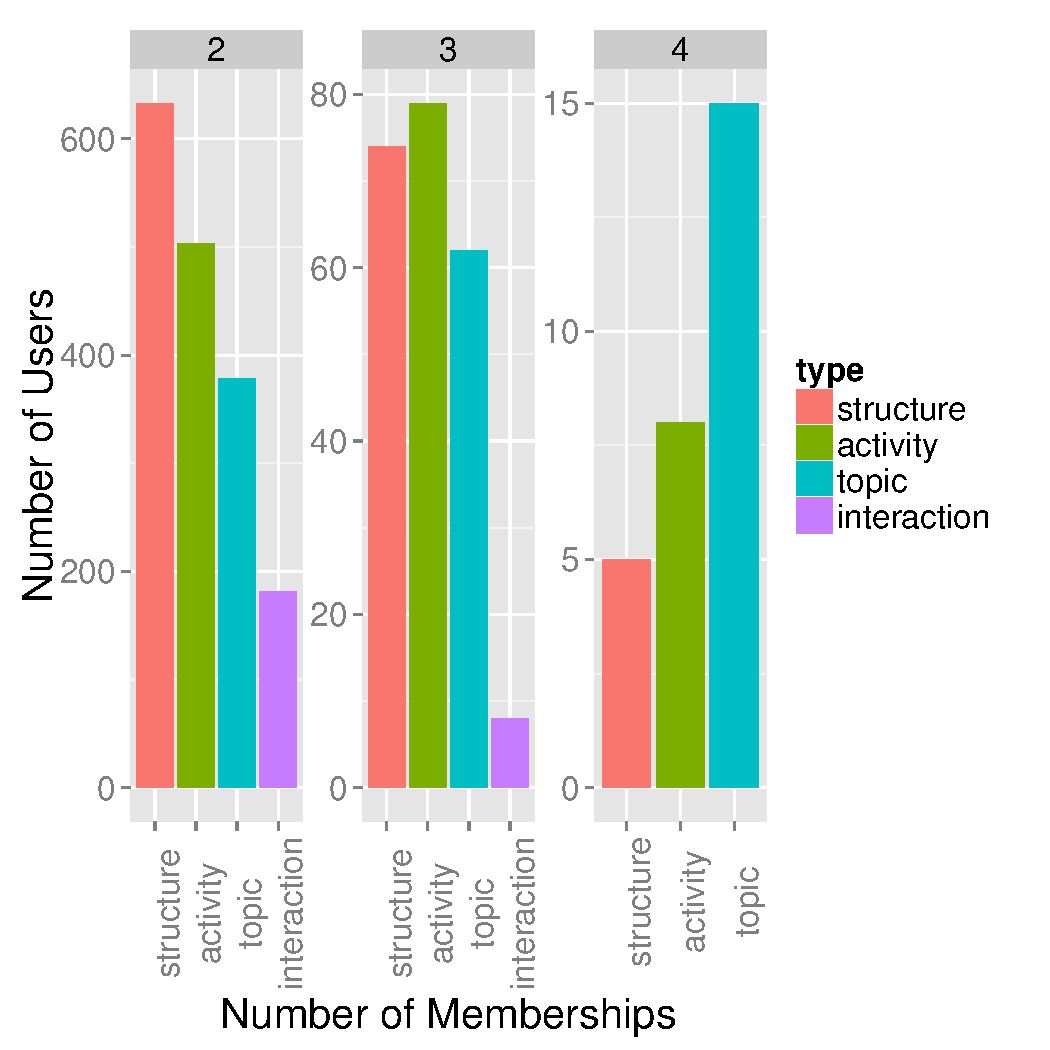
\includegraphics[width=0.50\textwidth]{Figures/overlap_by_type.pdf}
% \caption{The number of users belonging to 2, 3, or 4 communities, by community type.}
% \label{Fig-overlap_plot}
% \end{figure}

\subsection{Comparing Community Structure with Normalized Mutual Information}

In the previous section, we saw that the large scale statistics of the communities were highly dependent on the type of community under consideration. However, macroscale network statistics do not account for differences in community structure that result from operations such as splitting or merging of communities. Moreover, this view does not account for which users belong to which communities, and in particular which users belong to the same communities across community types. To answer this question, we invoke methods for the comparison of clusters: given two different clusterings of nodes into communities, how similar are the two clusters? The standard approach to answering this question is to define a metric on the space of possible partitions.  
Because we detect coverings rather than partitions, standard cluster comparison metrics like variation of information~\cite{meilua2003comparing} are not appropriate. Instead, we use a generalization of variation of information first introduced in~\cite{Lancichinetti2009}, the normalized mutual information. The normalized mutual information stems from treating clustering as a community identification problem: given that we know a node's community membership(s) in the first covering, how much information do we have about its community membership(s) in the second covering, and vice versa? Consider the two coverings $\mathcal{C}_{1}$ and $\mathcal{C}_{2}.$ We think of the community memberships of a randomly chosen node in $\mathcal{C}_{1}$ as a binary random vector $\mathbf{X} \in \{0, 1\}^{|\mathcal{C}_{1}|}$ where the $i^{\text{th}}$ entry of the vector is 1 if the node belongs to community $i$ and 0 otherwise. Similarly, $\mathbf{Y} \in \{ 0, 1\}^{|\mathcal{C}_{2}|}$ is a binary random vector indicating the community memberships of the node in $\mathcal{C}_{2}$. Then the normalized mutual information is defined as
\begin{align}
	\text{NMI}(\mathcal{C}_{1}, \mathcal{C}_{2}) = 1 - \frac{1}{2} \left( \frac{H[\mathbf{X} | \mathbf{Y}]}{H[\mathbf{X}]} + \frac{H[\mathbf{Y} | \mathbf{X}]}{H[\mathbf{Y}]}\right)
\end{align}
where $H[\cdot]$ denotes a marginal entropy and $H[\cdot | \cdot]$ denotes a conditional entropy. The normalized mutual information varies from 0 to 1, attaining the value of 1 only when $\mathcal{C}_{1}$ and $\mathcal{C}_{2}$ are identical coverings up to a permutation of their labels. See the appendix of~\cite{Lancichinetti2009} for more details.

We considered the normalized mutual information between the communities inferred from the structural network and the networks weighted with lag 1 through 6 transfer entropies, hashtag similarity, and mention, retweet, and mention-retweet activity. The resulting $\text{NMI}(\mathcal{C}_{i}, \mathcal{C}_{j})$ are shown in Figure~\ref{Fig-compare_coverings}. We see that similarity between the coverings is dictated by the generic community type (structural, activity-based, etc.). That is, the transfer entropy coverings are more similar to each other than to any of the other coverings, with a similar result for the mention, retweet, and mention-retweet coverings. Interestingly, the coverings resulting from the different weightings are all more similar to each other than to the structural covering from the unweighted network. Also note that the covering based on the hashtag similarities are different from all of the other weight-based coverings.

\begin{figure}[ht]
  \centering
  \begin{tabu}{cl}
    \toprule
    Normalized Mutual Information & Community Types \\
    \midrule
    \multirow{8}[8]{*}{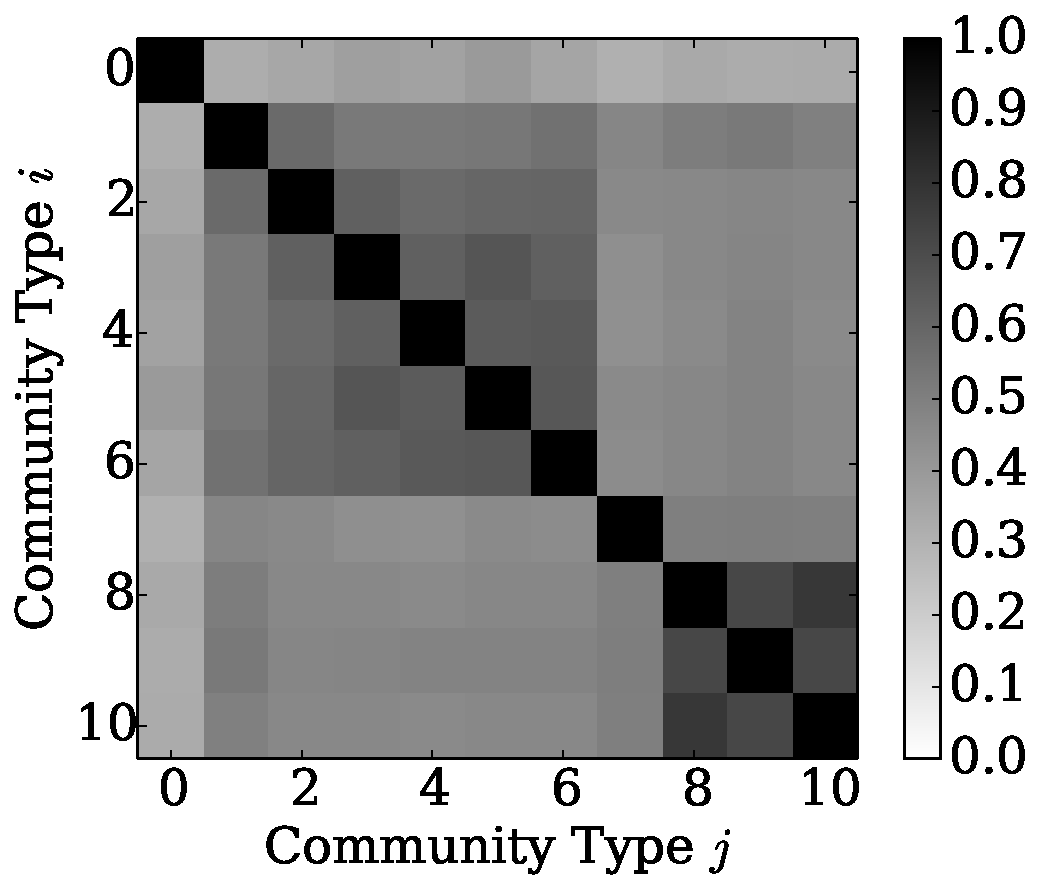
\includegraphics[width=0.50\textwidth]{nmi_singletons.pdf}}&0---Structural \bigstrut\\
    &1-6---Activity-Based with Lags 1-6\bigstrut\\
    %&2---Activity-Based with Lag 2\bigstrut\\
    %&3---Activity-Based with Lag 3\bigstrut\\
    %&4---Activity-Based with Lag 4\bigstrut\\
    %&5---Activity-Based with Lag 5\bigstrut\\
    %&6---Activity-Based with Lag 6\bigstrut\\
    &7---Topic-Based \bigstrut\\
    &8---Interaction-Based with Mentions\bigstrut\\
    &9---Interaction-Based with Retweets\bigstrut\\
    &10---Interaction-Based with both \bigstrut\\
    &\,\,\,\,\,\,\,\,\,\,\,\,\,\,Mentions and Retweets\bigstrut\\
    &\bigstrut\\
    \bottomrule
\end{tabu}
\caption{The normalized mutual information between the coverings inferred from the different community types. 
%Community type 0 corresponds to the structural communities, community types 1 through 6 correspond to the activity-based communities with lag 1 through 6 transfer entropies, community type 7 corresponds to the topic-based communities, and community types 8, 9, and 10 correspond to the interaction-based communities using mentions, retweets, and both mentions and retweets. 
Values of normalized mutual information close to 1 indicate similarity in the community structure, while values close to 0 indicate dissimilarity. The normalized mutual information is computed with singletons and orphan nodes included.}
\label{Fig-compare_coverings}
\end{figure}

Thus, we see that although the activity-based, interaction-based, and topic-based communities relied on the structural network, their community structure differs \emph{the most} from the community structure of the follower network. This agrees with the results from the previous section, and reinforces that the follower network is a necessary but not sufficient part of detecting communities characterized by properties beyond follower-followee relationships.

%%%%%%%%%%%%%%%%%%%%%%%%%%%%%%%%%%%%%%%%%%%%%%%%%%%%%%%%%%%%% 
%============================================================
% Old section on 'Comparing Edges Across Different Community Types'

% \subsection{Comparing Edges Across Different Community Types}

% We next explore how the edge weights defined by equations (\ref{Eqn-EW-activity}), (\ref{Eqn-EW-interaction}), and (\ref{Eqn-EW-topic}), and thus different forms of information flow, differ between community types. For a fixed community type, edges for a particular community may be partitioned into three sets: those from a user in the community to another user in the community (internal-to-internal), those from a user in the community to a user outside of the community (internal-to-external), and those from a user outside the community to a user inside the community (external-to-internal). See Figure~\ref{Fig-edge_types} for a schematic of this edge partitioning. For a meaningful community, we expect the distribution of weights within the community (internal-to-internal weights) to be different from the distribution of weights without the community (internal-to-external and external-to-internal).

% \begin{figure}[ht]
%   \centering
% 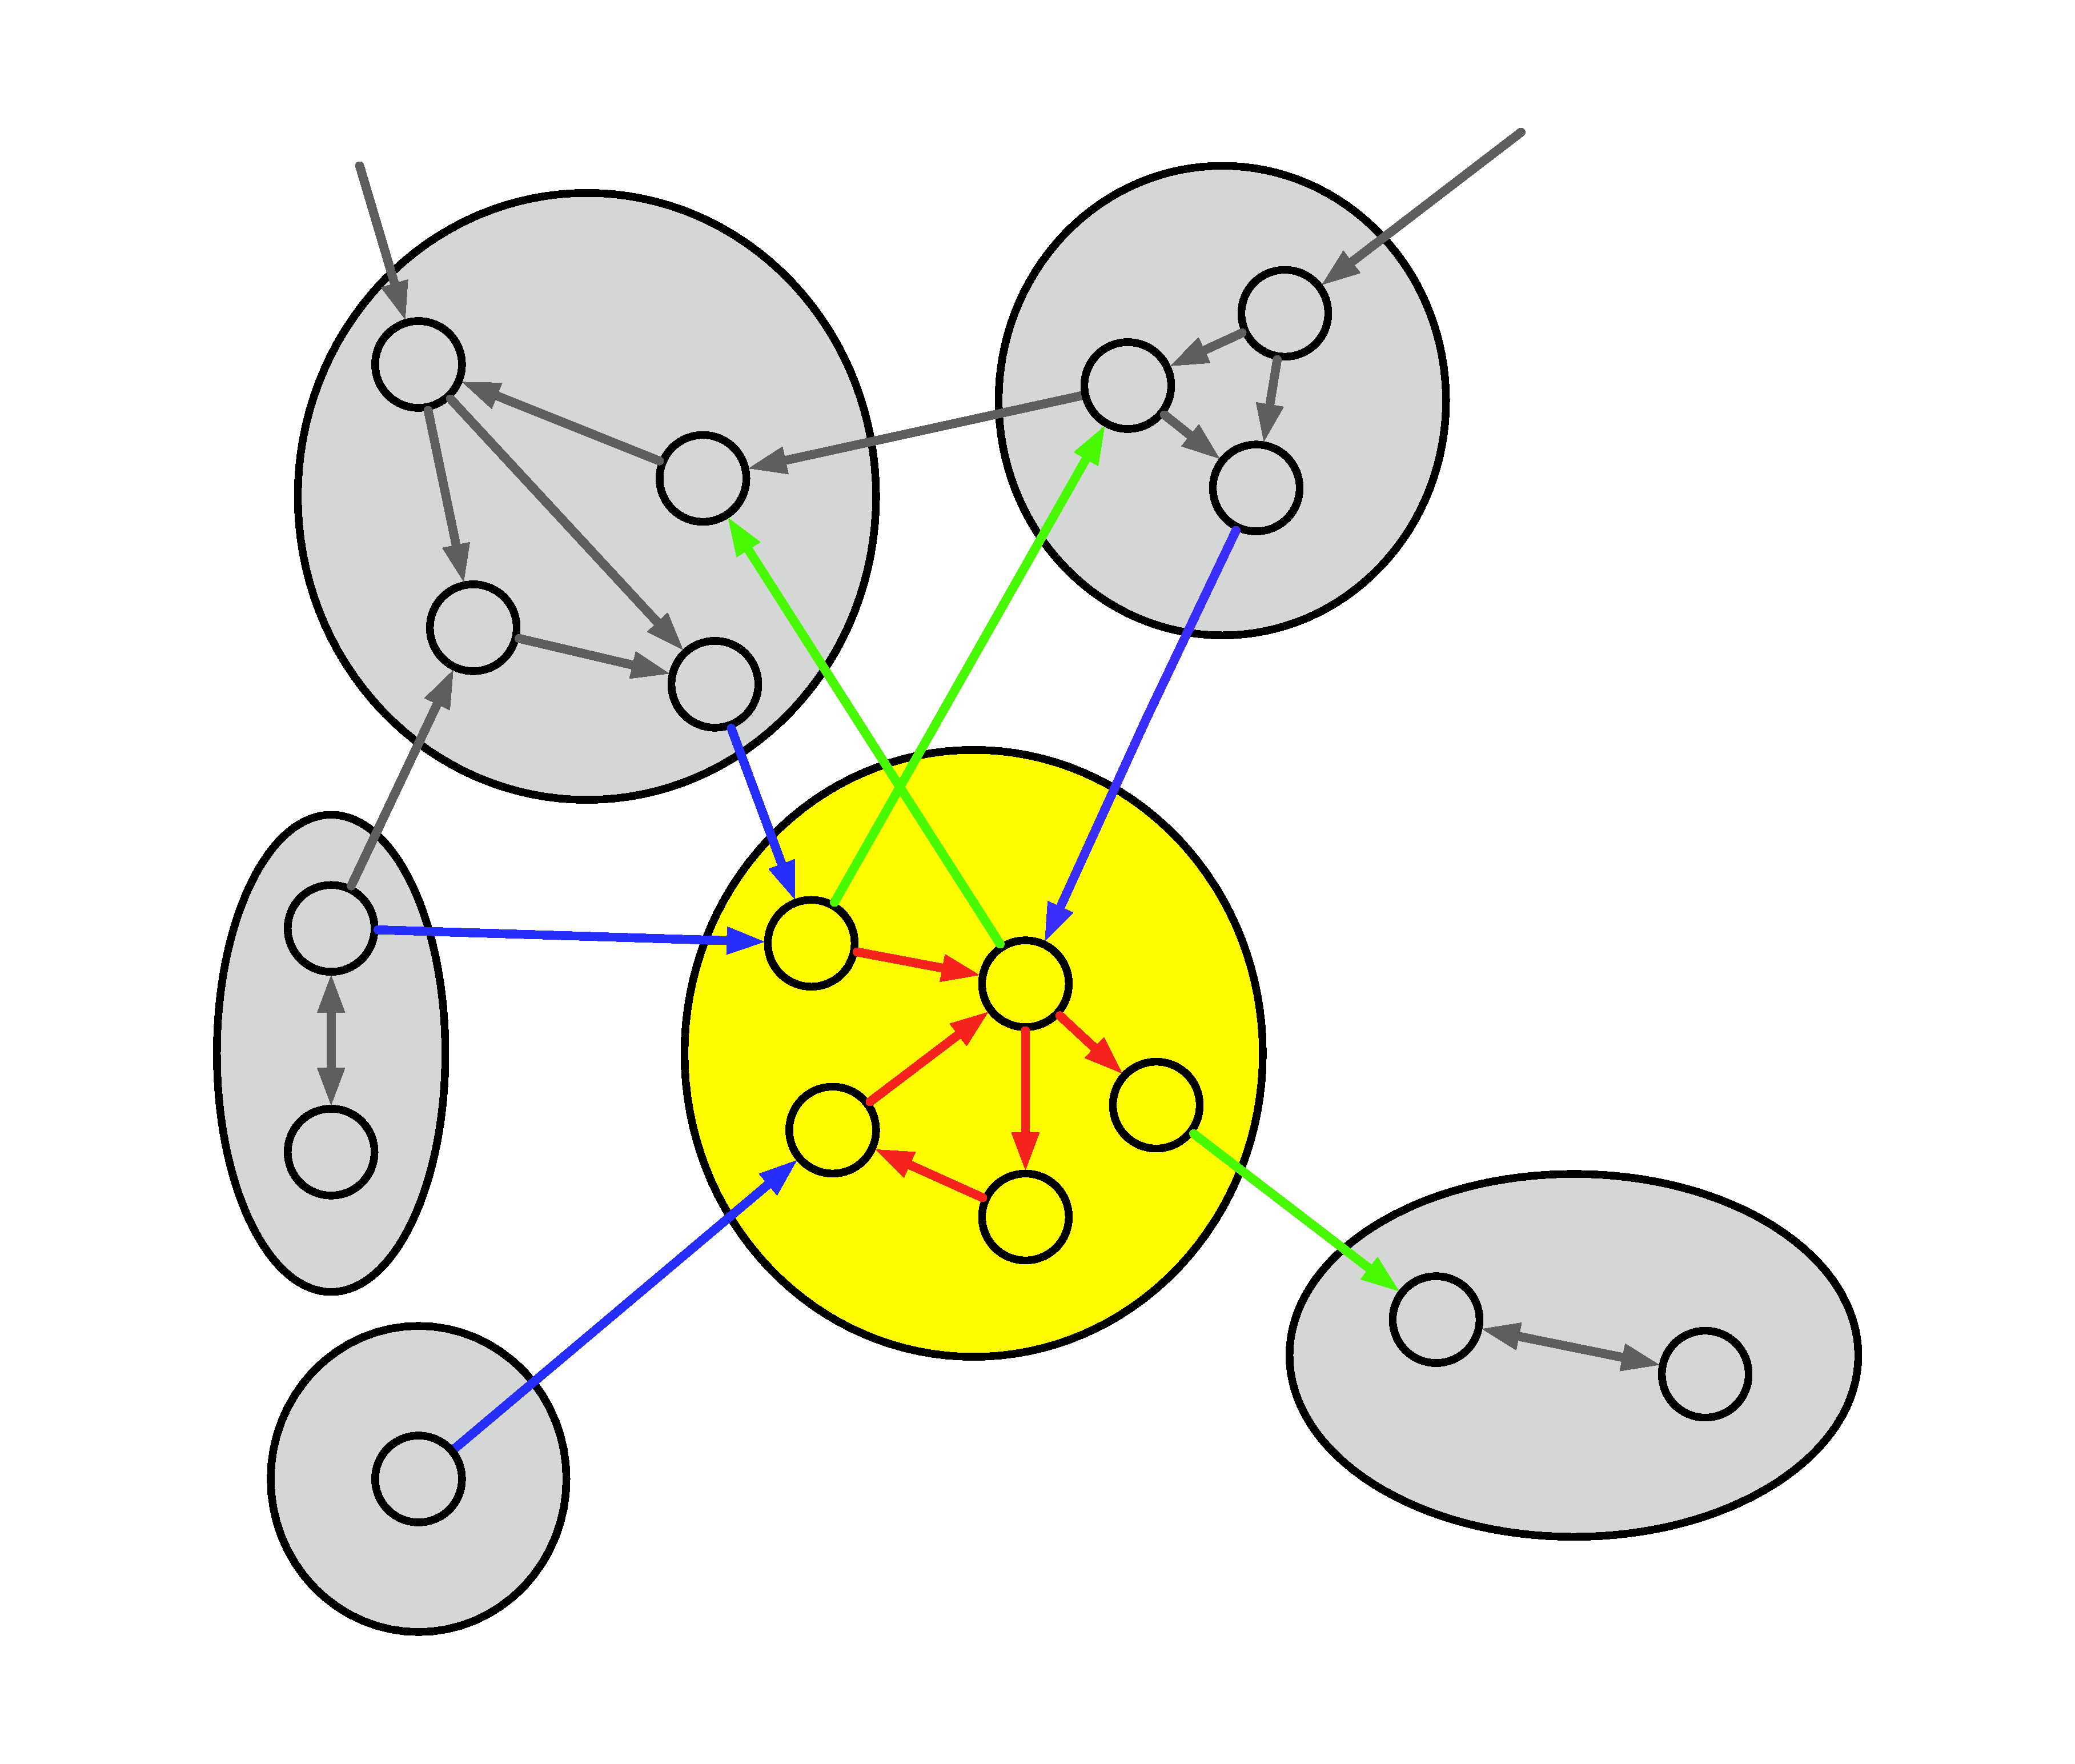
\includegraphics[width=0.50\textwidth]{edge-types.eps}
% \caption{An example of the edges considered in determining the edge weight distribution for a given community (the focal community is in yellow). We focus on the internal-to-internal (red), internal-to-external (green), and external-to-internal (blue) edges. For a given focal community, all other edges (grey) are not considered.}
% \label{Fig-edge_types}
% \end{figure}

% As an example, Figure~\ref{Fig-dist_across_community} shows the distributions of hashtag-based weights for the largest community in the mention-retweet network. We see that the distribution of internal-to-internal hashtag weights has a longer tail than either the external-to-internal or internal-to-external hashtag weights, with edges within the community having higher weights than edges crossing the boundary of the community. Thus, while the community was defined in terms of interactions, we still see a shift in the distribution of topic-similarity.

% \begin{figure}[ht]
%   \centering
% 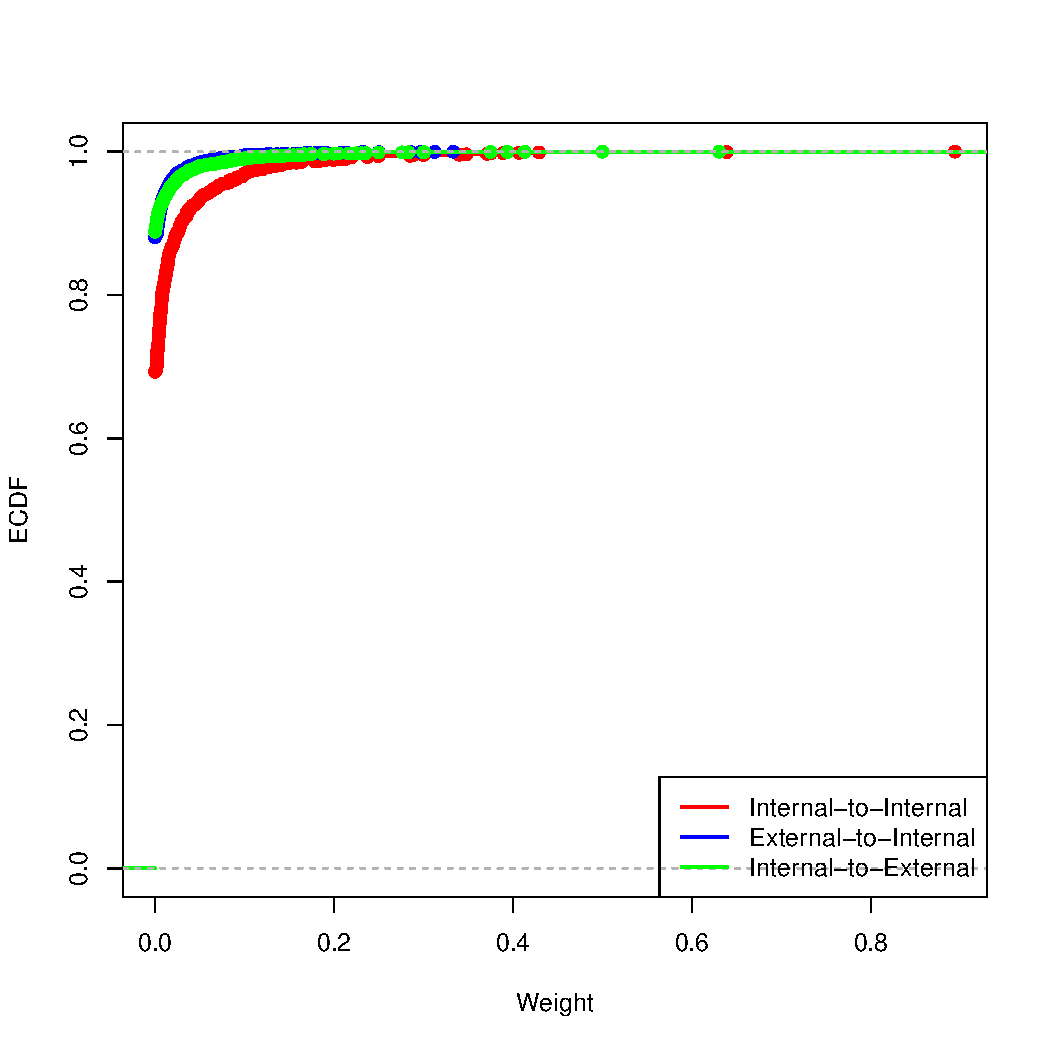
\includegraphics[width=0.50\textwidth]{comm0_labels-hashtag_weights-mention-retweet-ecdf.pdf}
% \caption{The proportion of edges with a weight at least as large as the weight on the horizontal axis, across the types of edges described in Figure~\ref{Fig-edge_types}. The community is defined by user interactions, and the edge weights are determined by topic similarity. The dashed vertical lines indicate the median weight for each type of edge. Note the logarithmic scale on the horizontal axis.}
% \label{Fig-dist_across_community}
% \end{figure}

% \begin{figure}
%         \centering
%         \begin{subfigure}[b]{0.2\textwidth}
%                 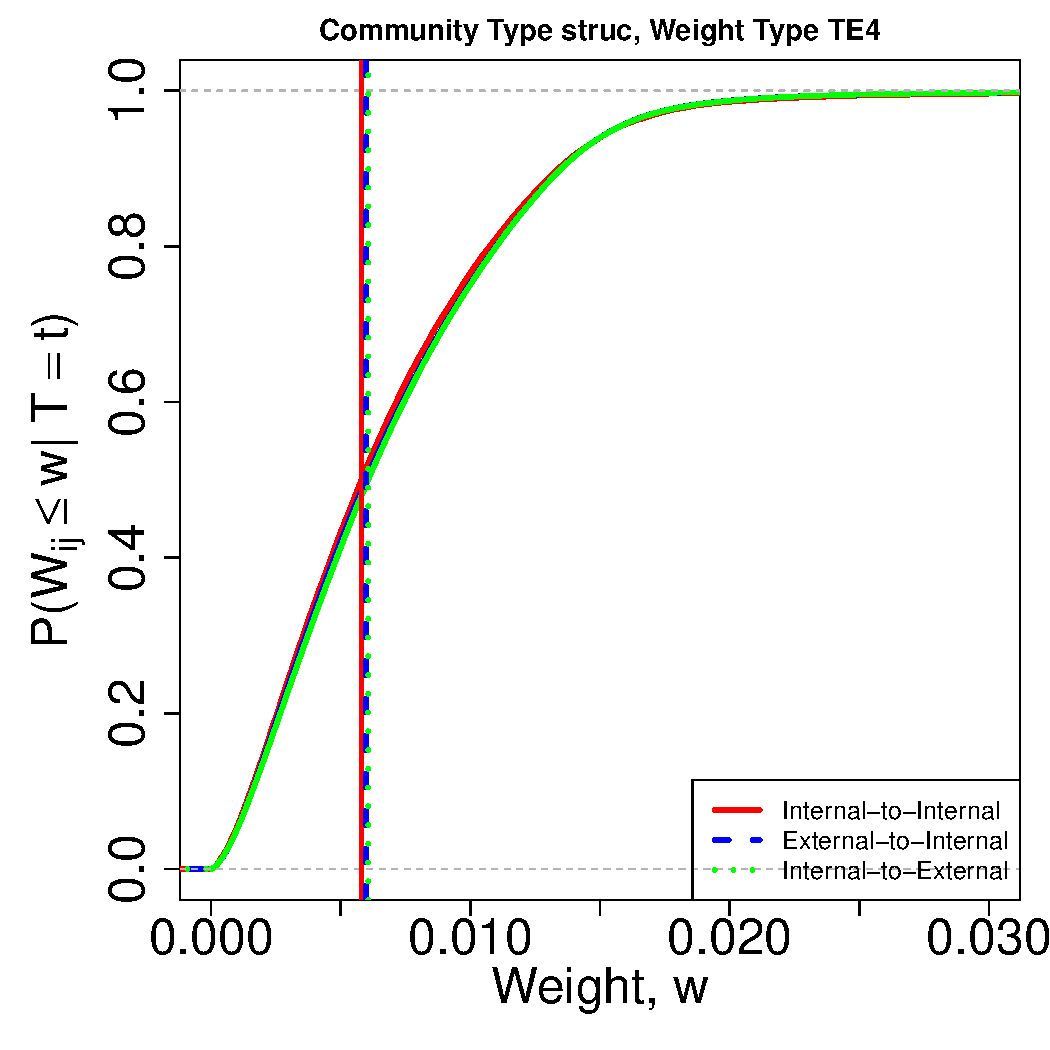
\includegraphics[width=\textwidth]{labels-struc_weights-TE4-ecdf_by_type.pdf}
%         \end{subfigure}
%         \begin{subfigure}[b]{0.2\textwidth}
%                 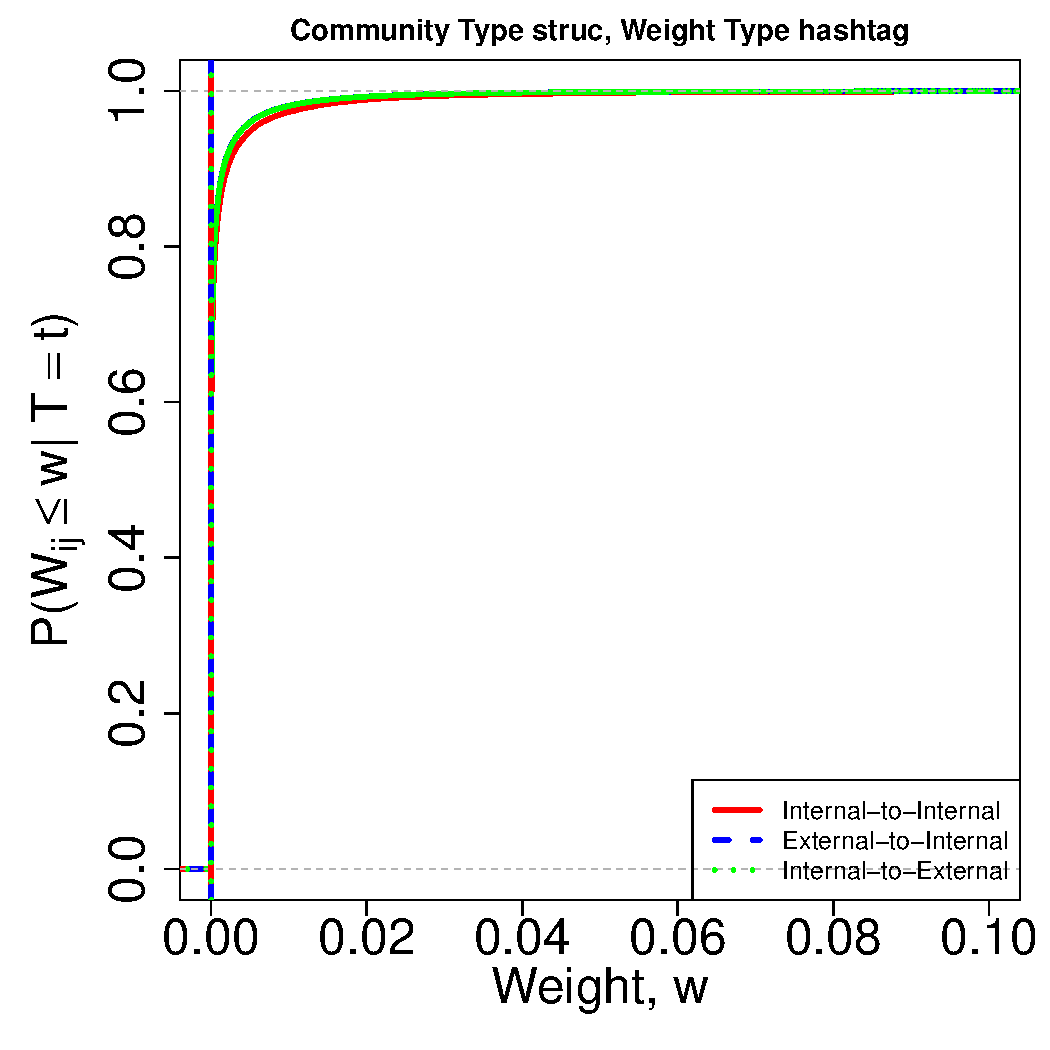
\includegraphics[width=\textwidth]{labels-struc_weights-hashtag-ecdf_by_type.pdf}
%         \end{subfigure}
%         \begin{subfigure}[b]{0.2\textwidth}
%                 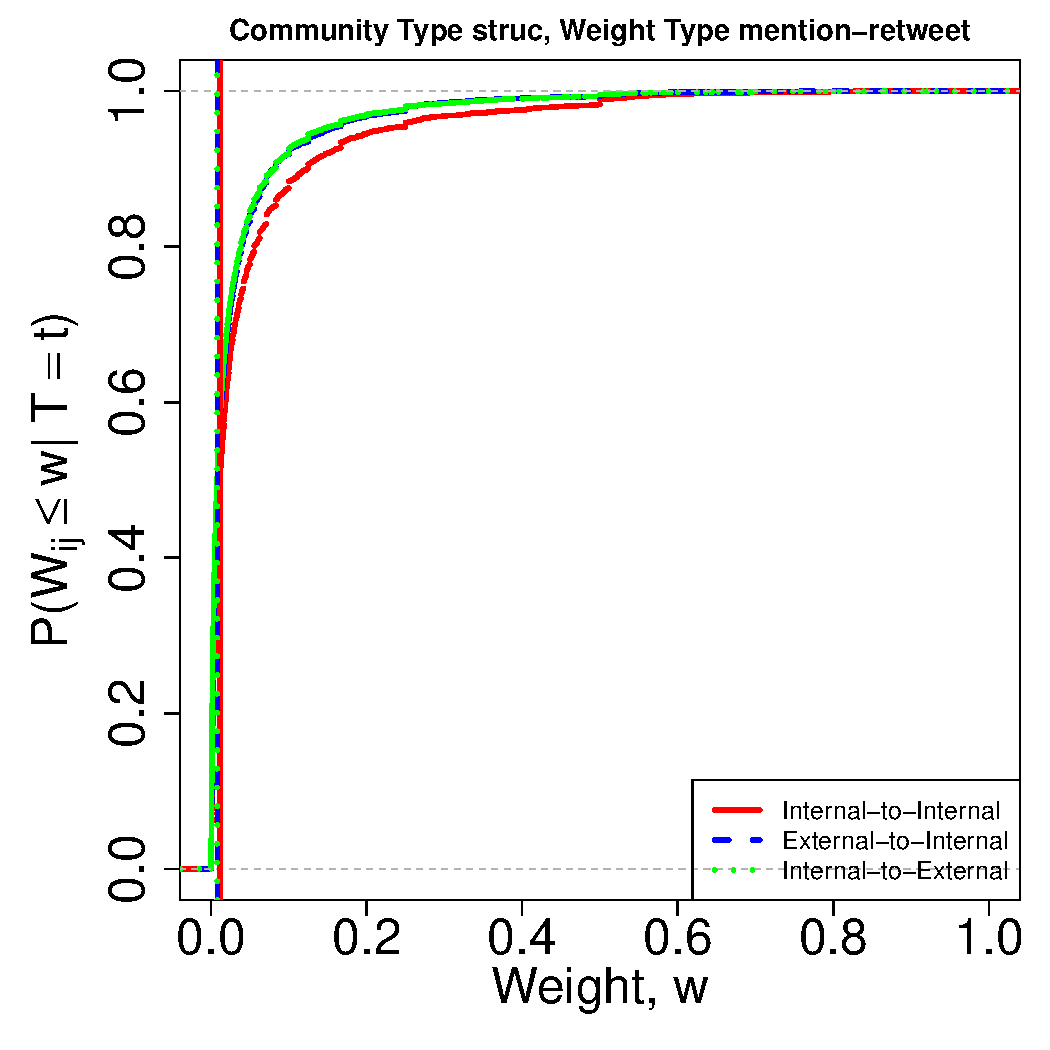
\includegraphics[width=\textwidth]{labels-struc_weights-mention-retweet-ecdf_by_type.pdf}
%         \end{subfigure}
%         \caption{Lorem ipsum.}
% \end{figure}

% This change in the tail of the distribution between edge types was typical of many of the community type / weight pairings. A useful summary statistic to quantify the change involves the median weights across the three types of edges, as demonstrated in Figure~\ref{Fig-dist_across_community}. In particular, by computing the ratio of the median weight for the internal-to-internal edges to the median weight for the internal/external-to-external/internal edges, we can quantify the ratio change in weight strength internal vs. external to a community. We computed this quantity for each of the top 100 largest communities defined by a particular community type (structure-based, activity-based, interaction-based, or topic-based), and report the median value across the 100 largest communities for each type in Table~\ref{Table-medians}. This statistic represents the typical ratio shift for each community type / weight pairing. Values greater than 1 indicate that the edge weights tend to be higher within the community, and values less than 1 indicate that the edge weights tend to be higher for those edges crossing the community boundary.

% \begin{table}
% 	\caption{The median value for the ratio of the median external/internal-to-internal/external weight to median internal-to-internal weight for the different community/weight pairings.}
% 	\centering
% 	\begin{tabular}{c | c | c  c  c  c}
% 		& & \multicolumn{4}{ c }{Community} \\ \hline
% 		\multirow{4}{*}{Weight} & & S & TE & MR & HT \\ \hline
% 		& TE & $0.0 / 0.0$ & $0.0 / 0.0$ & $0.0 / 0.0$ & $0.0 / 0.0$\\
% 		& MR & $0.0 / 0.0$ & $0.0 / 0.0$ & $0.0 / 0.0$ & $0.0 / 0.0$\\
% 		& HT & $0.0 / 0.0$ & $0.0 / 0.0$ & $0.0 / 0.0$ & $0.0 / 0.0$
% 	\end{tabular}
% \end{table}

% \begin{table}
% 	\label{Table-medians}
% 	\caption{The median value across the 100 largest communities for the ratio of the median internal-to-internal weight to the median external-to-internal / internal-to-external weight for the different community / weight pairings. Note: For mention-retweet weights, weight zero edges were excluded from the computation of the median. We indicate such cases with an asterisk.}
% 	\centering
% 	\begin{tabular}{c | c | c  c  c}
% 		& & \multicolumn{3}{ c }{Weight Type} \\ \cline{3-5}
% 		& & TE & MR & HT \\ \cline{2-5}
% 		\multirow{4}{*}{Community Type} & S & $0.96/0.94$& $1.7/2.1$*& $9.0/8.0$\\
% 		& A & $1.0/0.96$& $1.5/2.4$*& $24/17$\\
% 		& I & $0.83/0.86$& $3.2/4.4$& $10/8.5$\\
% 		& T & $0.9/0.89$& $2.4/2.6$*& $28/26$
% 	\end{tabular}
% \end{table}

% \begin{table}
% 	\caption{The median value across the 100 largest communities for the ratio of the median internal-to-internal weight to the median external-to-internal / internal-to-external weight for the different community / weight pairings. For each entry $a/b$ in the table, $a$ corresponds to median ratio value for edges external-to-internal, and $b$ corresponds to the median ratio value for edges internal-to-external . Community types correspond to S(tructural), A(ctivity-based), T(opic-based), and I(nteraction-based) communities. Weight types correspond to T(ransfer) E(ntropy), M(ention-)R(etweet), and H(ash)T(ag). Note: For mention-retweet weights, zero weight edges were excluded from the computation of the median. We indicate such cases with an asterisk.}
% 	\centering
% 	\begin{tabular}{c  c | c  c  c}
% 		& & \multicolumn{3}{ c }{Weight Type} \\ %\cline{3-5}
% 		& & TE & MR & HT \\ \cline{1-5}
% 		\multirow{4}{*}{Community} & S & $0.96/0.94$& $1.7/2.1$*& $9.0/8.0$\\
% 		\multirow{4}{*}{Type} & A & $1.0/0.96$& $1.5/2.4$*& $24/17$\\
% 		& I & $0.83/0.86$& $3.2/4.4$& $10/8.5$\\
% 		& T & $0.9/0.89$& $2.4/2.6$*& $28/26$
% 	\end{tabular}
% 	\label{Table-medians}
% \end{table}

% We see that for every weight type except transfer entropy, the weight on edges internal to the communities tend to be higher than on edges entering or exiting the communities, ranging from a factor of 1.5 times larger for the activity-based/mention-retweet pairing to a factor of 28 times larger for the topic-based/hashtag similarity pairing. As stated above, we expect this ratio to be high for community / weight pairings that match (e.g. considering mention-retweet weighting for interaction-based communities), and we see that this is the case for all but the activity-based / transfer entropy pairing. Moreover, for both the mention-retweet and hashtag weightings, the ratio is largest when they match with the interaction-based and topic-based communities, respectively.

% For all four community types, the transfer entropy tended to be higher for edges crossing community boundaries than for those internal to community boundaries. Recall that the transfer entropy $\text{TE}_{X(u) \to X(f)}$ quantifies the reduction in uncertainty about a follower $f$'s activity from knowing the activity of a user $u$. This result therefore implies that, in terms of prediction, it is more useful to know the time series of a user followed outside of the community compared to a user followed inside of the community. Thus, in an information theoretic sense, we see that novel information useful for prediction is more likely to flow \emph{across} community boundaries than \emph{within} community boundaries.

% Note that the communities defined by the follower network do tend to have higher edge weights internal compared to across community boundaries. Thus, we do see that the structural communities capture some information about the functional behavior of communities of users in terms of topics and interaction. However, the ratio is not as large as when we explicitly seek out communities based on a particular type of functional community. This again emphasizes the importance of properly formulating the goal of a community detection study in the context of online social networks.

% \begin{tabular}{cc|ccc}
% & & \multicolumn{3}{ c| }{Weight Type} \\ \cline{3-5}
% & & 2 & 3 & 5  \\ \cline{1-5}
% \multicolumn{1}{ c| }{\multirow{4}{*}{Powers} } &
% \multicolumn{1}{ c| }{504} & 3 & 2 & 0    \\ \cline{2-5}
% \multicolumn{1}{ c|  }{}                        &
% \multicolumn{1}{ c| }{540} & 2 & 3 & 1     \\
% \multicolumn{1}{ c| }{gcd} & 2 & 2 & 0 \\ \cline{2-5}
% \multicolumn{1}{ c  }{}                        &
% \multicolumn{1}{ c| }{lcm} & 3 & 3 & 1 \\ \cline{1-5}
% \end{tabular}

%%%%%%%%%%%%%%%%%%%%%%%%%%%%%%%%%%%%%%%%%%%%%%%%%%%%%%%%%%%%% 
%============================================================

%%%%%%%%%%%%%%%%%%%%%%%%%%%%%%%%%%%%%%%%%%%%%%%%%%%%%%%%%%%%% 
%============================================================
% New section on 'Comparing Edges Across Different Community Types'

\subsection{Comparing Edges Across Different Community Types}

Any covering determined by OSLOM induces a natural partition of the edges in a directed network. In particular, Let $u$ and $f$ be two users in the network, and let $M_{u}$ and $M_{f}$ be their community memberships. Then any edge $e_{u \to f}$ can be partitioned into one of three classes by
\begin{align}
	T(e_{u \to f}) = \left\{ \begin{array}{ll}
		\text{Inter-edge} &: \ \ \ M_{u} \cap M_{f} = \emptyset \\
		\text{Intra-edge} &: \ \ \ M_{u} = M_{f}\\
		\text{Mixed-edge} &: \ \ \ \text{ otherwise} \\
	\end{array}\right. \label{Eqn-edge_types}.
\end{align}
In words, an inter-edge connects two users who share no community memberships, an intra-edge connects two users who each belong to the same communities, and a mixed-edge connects two users who share some, but not all, community memberships. Thus, inter-edges cross community boundaries, intra-edges lie within community boundaries, and mixed-edges lie at the borders of community boundaries. See Figure~\ref{Fig-edge_types} for a schematic of this edge partitioning.

\begin{figure}[!h]
	\centering
	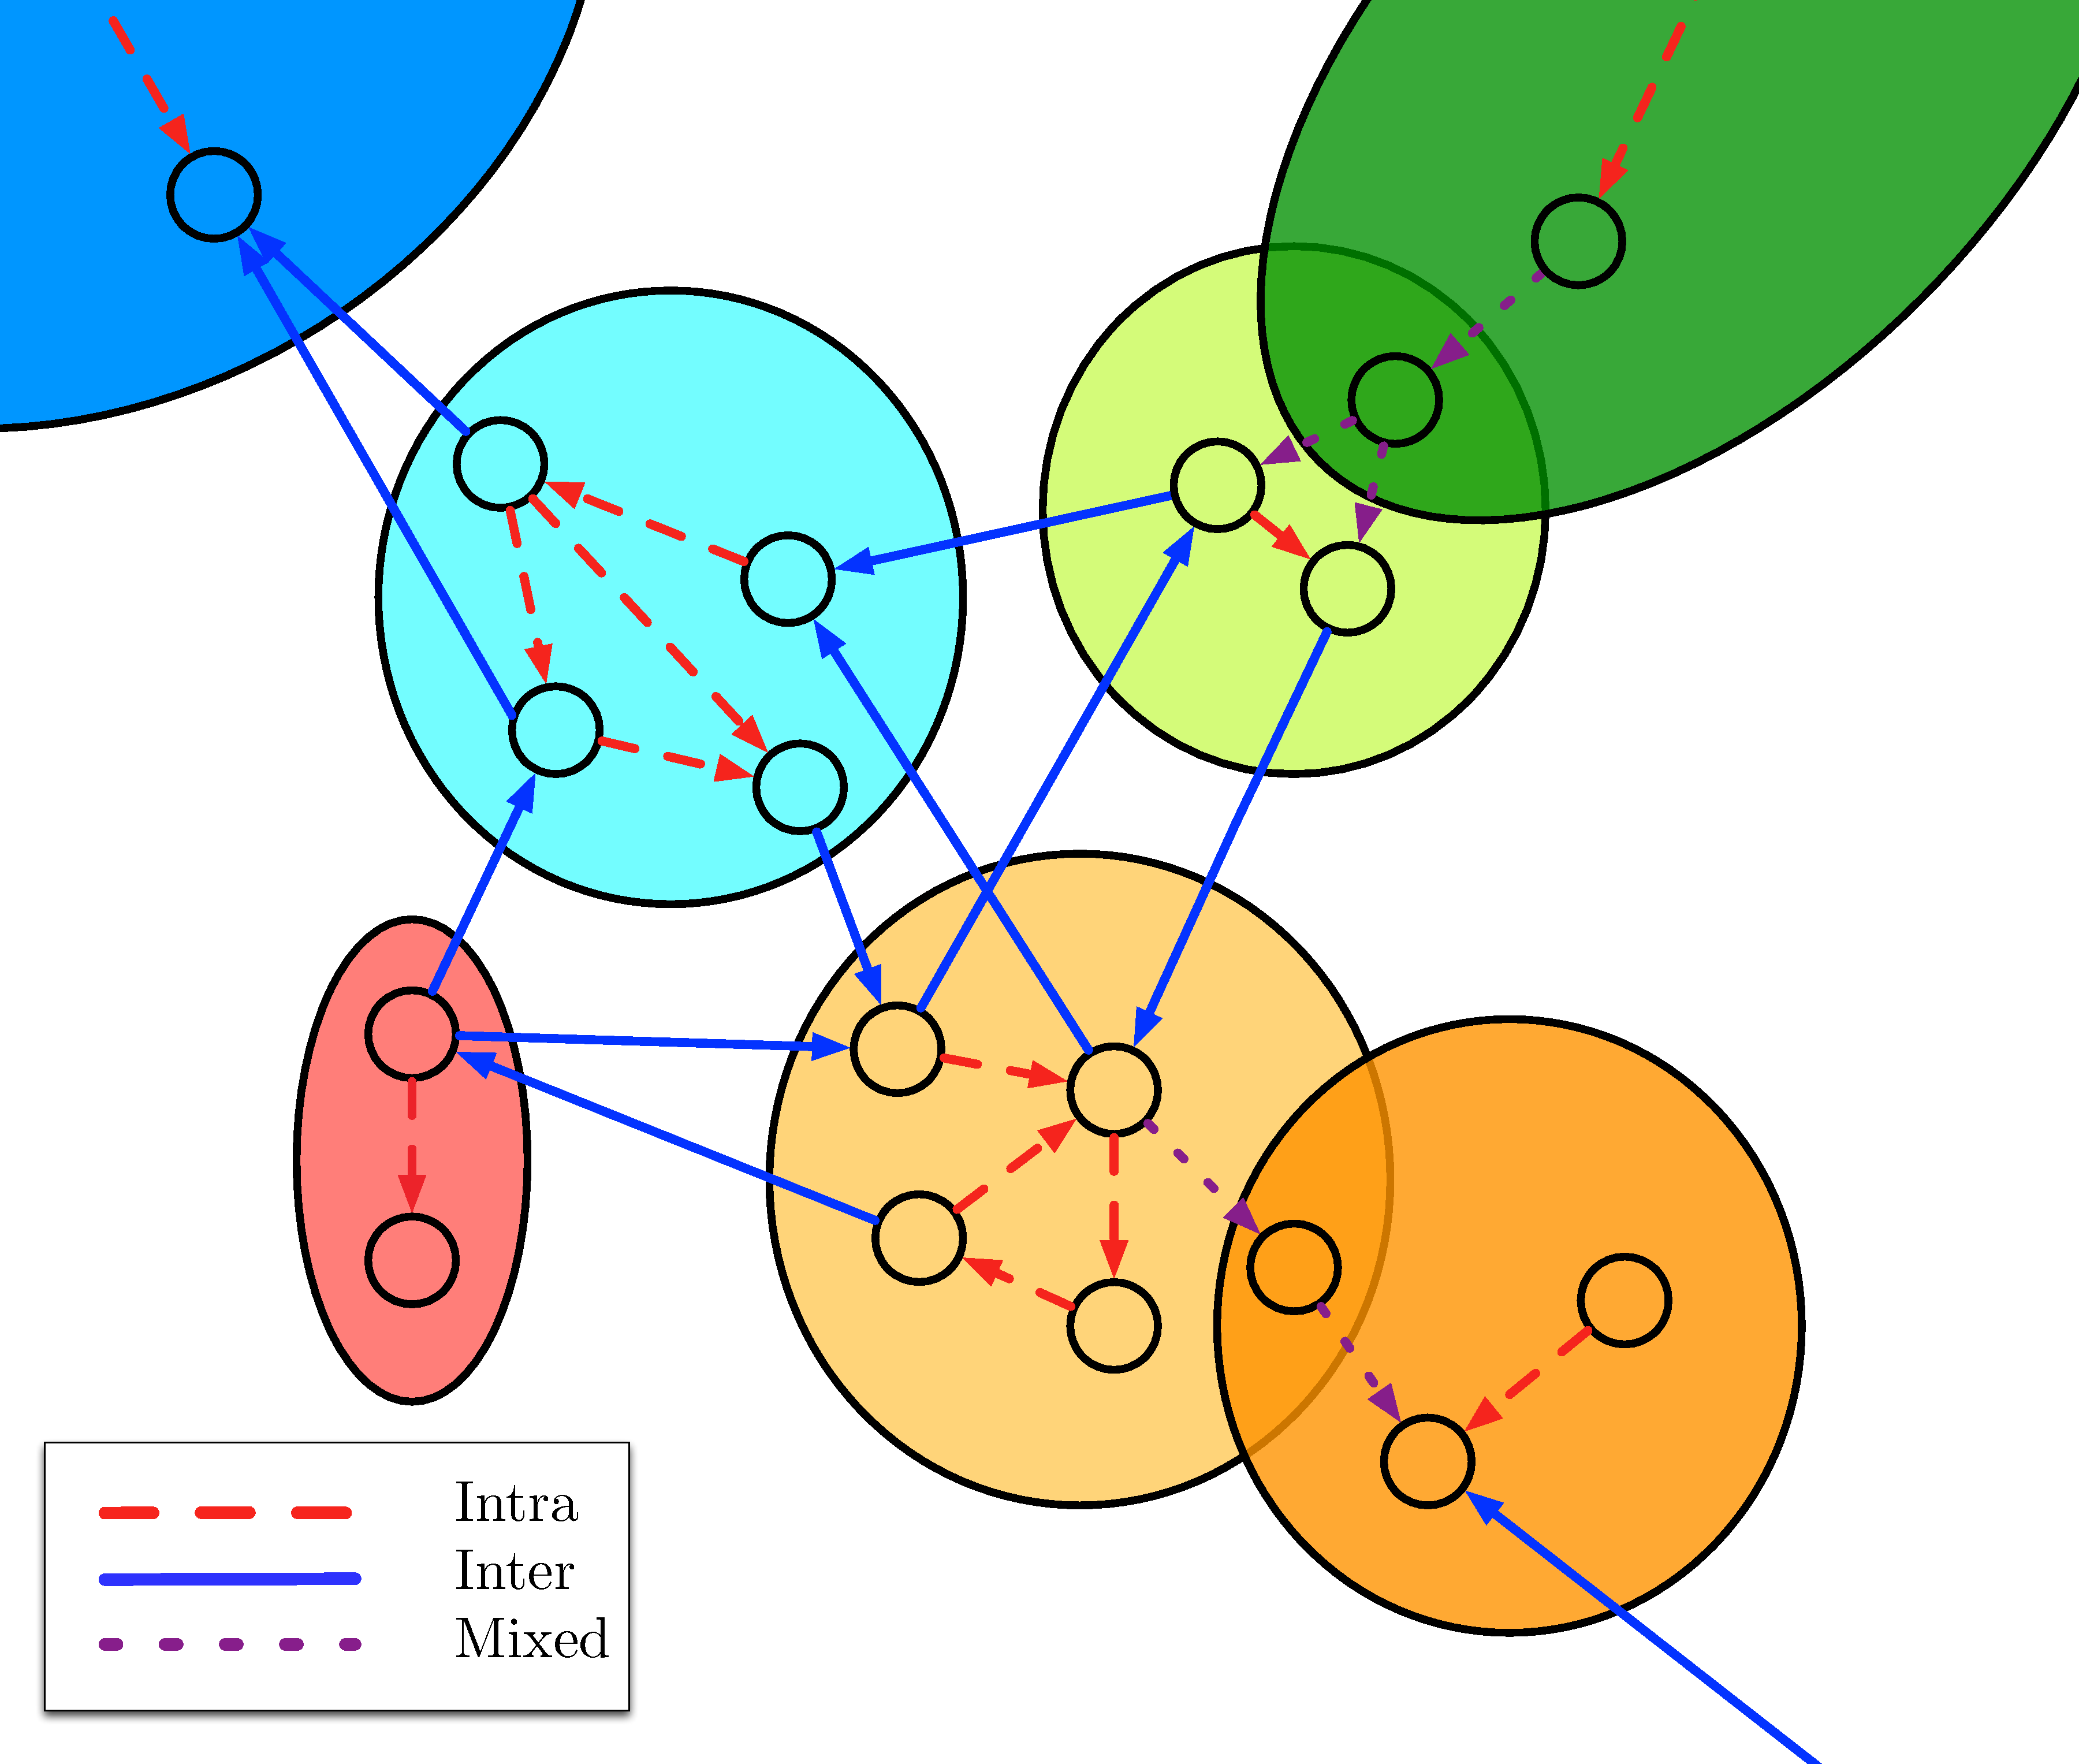
\includegraphics[width=0.8\textwidth]{edge-types.pdf}
	\caption{A schematic of how, given a covering, the edges of the network can be partitioned using \ref{Eqn-edge_types} into inter-edges, intra-edges, and mixed-edges. Inter-edges (red) cross community boundaries. Intra-edges (blue) remain inside community boundaries. Mixed-edges (purple) both remain in and cross community boundaries due to overlap in community membership. Each column corresponds to the same collection of weights, but partitioned using a different covering. Each row corresponds to the same covering, but for the different weights.}
	\label{Fig-edge_types}
\end{figure}

\begin{table}
	\caption{The percentage of intra-, inter-, and mixed-edges associated with the coverings for each of the four community types.}
	\centering
	\begin{tabular}{l | r r r}
		Community Type & Intra & Inter & Mixed \\
		\hline
		Structural & 7.5 & 87.0 &  5.5 \\
		Activity-based & 10.7 & 81.9 & 7.4 \\
		Topic-based & 7.3 & 89.0  & 3.7 \\
		Interaction-based & 42.3 & 47.9 & 9.8
	\end{tabular}
\end{table}

Each community type (Structural, Activity-based, Topic-based, Interaction-based) induces a different partition of the edges, and each edge type (Transfer Entropy, Hashtag, Mention-Retweet) induces a different distribution of weights. That is, let $W_{u \to f}$ be the weight on a randomly selected edge $E_{u \to f}$ from the network, and compute
\begin{align}
	P(W_{u \to f} \leq w | T(E_{u \to f}) = t),
\end{align}
the empirical distribution over the edge weights conditioned on $t$ being one of inter, intra, and mixed. For meaningful community structure, we expect the distribution of edge weights to differ with the edge type $t$. If the community structure were arbitrary, the edge weights would be independent of the edge type, and all three conditional distributions would be identical.
The densities associated with these distributions are shown in Figure~\ref{Fig-distributions_by_types}, included in Appendix B.

Each \emph{column} of Figure~\ref{Fig-distributions_by_types} demonstrates how the density of weights change with the community type used to induce the partition. For example, the second column shows how the density of hashtag weights change based on the community partition. In general, the densities differ in non-trivial ways across the edge types and coverings. However, we see that the medians of the distributions provide a useful summary statistic. Under each collection of density functions, we list the median value of the inter, intra, and mixed-edges in red, blue, and magenta, respectively. Unsurprisingly, we see that the greatest difference between the distributions occurs when we consider the topic-based communities, since the topic-based communities are determined based on the hashtag weights. However, we also see differences in the distributions when the Community-type / Weight-type pairs do not match. For example, for the covering corresponding to the activity-based communities, the hashtag weights tend to be higher for edges internal to communities than between communities. Similarly, for the covering corresponding to the topic-based communities, the transfer entropy weights tend to be higher on edges within (intra) and between (inter) communities, and lower for edges between members with multiple, non-identical memberships (mixed).

We also note that the distribution of transfer entropy weights always tend to be higher for edges crossing community boundaries (inter- or mixed-edges) compared to those edges within community boundaries (intra-edges). This is a property not exhibited by either the hashtag or mention-retweet weights, independent of the covering used to partition the edges. Moreover, for all but the activity-based covering, the weights of mixed-edges tend to be highest overall.  Recall that the transfer entropy $\text{TE}_{X(u) \to X(f)}$ quantifies the reduction in uncertainty about a follower $f$'s activity from knowing the activity of a user $u$. This result therefore implies that, in terms of prediction, it is more useful to know the time series of a user followed outside of the community compared to a user followed inside of the community, and even more useful to know the time series of a user that shares some, but not all, of the same community memberships. Thus, in an information theoretic sense, we see that novel information useful for prediction is more likely to flow \emph{across} community boundaries than \emph{within} community boundaries.

% \subsection{Demonstration of the Question-Oriented Approach}
%
% Next, we demonstrate a particular instance of a question-oriented approach. Suppose we were interested in tracking where conversations occur in a social network. That is, we want to track groups of individuals who interact more with each other than with users outside of their group. For example, we might wish to select a seed group of individuals in order to spread a message to a subpopulation of a social network. We now demonstrate how the performance on this tracking problem depends on the community type under consideration.
%
% % * We want to track *where* conversations are occurring: amongst what group of people.
%
% % * This motivates using the interaction-based communities.
%
% The data set was divided into two disjoint time periods: from 9am April 25th 2011 to 9am May 23rd 2011 (28 days) and from 9am May 23rd 2011 to 9am June 25th 2011 (33 days). We then constructed the three weighted networks (the structural network is unchanged) using the activity, retweets, mentions, and hashtags from the first time period, as described in the methodology section. Using the coverings inferred by OSLOM for the weighted network, we define the inside and outside of a community in the same way as depicted in Figure~\ref{Fig-edge_types}, where now we consider mixed-type edges to be internal. Based on this partitioning of the edges, we then track how many of the retweets / mentions in the second time period fall inside vs outside of the communities. The percentages of retweets and mentions that occur internal to each of the community types are given in Table~\ref{Tab-mentionretweets}.
%
% \begin{table}
% 	\caption{The percentage of retweets and mentions that occur internal to communities for each of the four community types.}
% 	\centering
% 	\begin{tabular}{l | c c}
% 		Community Type & Percentage of Retweets Internal & Percentage of Mentions Internal \\
% 		\hline
% 		Structural & 47.5 & 70.9 \\
% 		Activity-based & 54.7 & 75.6 \\
% 		Topic-based & 49.4 & 66.8  \\
% 		Interaction-based & \textbf{67.2} & \textbf{84.2}
% 	\end{tabular}
% 	\label{Tab-mentionretweets}
% \end{table}
%
% Let $I_{c}$ be the number of conversations (defined as a retweet or mention) occuring internal to community $c$, and let $|\mathcal{C}|_{c}$ be the size of community $c$. Finally, let $N$ be the total number of conversations, both internal and external, involving the nodes. An alternative scoring function is then
% \begin{align}
% 	\frac{1}{N}\sum_{c} \frac{I_{c}}{|\mathcal{C}_{c}|}.
% 	\label{conversation-metric}
% \end{align}
% That is, this measures the average number of internal conversations per user in a community. This will be maximized when the communities are small and the number of internal conversations are large compared to the total number of conversations.
%
% \begin{table}
% 	\caption{The metric (\ref{conversation-metric}) for the four community types, computed using the held-out data.}
% 	\centering
% 	\begin{tabular}{l | c c}
% 		Community Type & Retweets & Mentions \\
% 		\hline
% 		Structural & 0.0289 & 0.0344 \\
% 		Activity-based & 0.0793 & 0.0645 \\
% 		Topic-based & 0.1031 & 0.1020  \\
% 		Interaction-based & 0.0690 & 0.0977
% 	\end{tabular}
% 	\label{Tab-mentionretweets2}
% \end{table}
%
% \begin{table}
% 	\caption{The value of the conversation metric proposed by Elisa, averaged over all of the communities in a given covering.}
% 	\centering
% 	\begin{tabular}{ l | c c}
% 		Community Type & Mentions & Retweets \\
% 		\hline
% 		Structural & 2.9347 & 0.4734 \\
% 		Activity-based & \textbf{3.3893} & 0.5173 \\
% 		Topic-based & 2.5944 & 0.5580 \\
% 		Interaction-based & 2.1984 & \textbf{1.1069}
% 	\end{tabular}
% \end{table}

\subsection{Qualitative Analysis of Community Memberships Across Types}

As demonstrated by~\cite{good2010performance} in the context of modularity maximization-based community detection, an exponential number of nearby partitions may exist that nearly maximize an objective function used to measure the goodness-of-fit of a graph partition used for community detection. Because of this and related issues, it is always wise to perform some sort of qualitative study of the communities returned by any  community detection algorithm to verify their meaningfulness with respect to the scientific question at hand. In this section, we consider a collection of communities in such a study. 

In the topic-based communities, we find a single community consisting of 83 users who tweet about environmental issues and frequently use hashtags such as \#green, \#eco and \#sustainability. We also find a different community of 47 users who tweet about small businesses and entrepreneurship, using hashtags such as \#smallbiz, \#marketing and \#enterpreneur. In both cases most members of the topic-based communities are not found in the same community in the other networks, indicating that while these people talk about the same things and can therefore be considered a community based on their content, they do not strongly interact with each other nor behave the same, and so belong to different social groups with respect to interactions and behavior.

Another interesting example is a community whose topics tend to focus on Denver and Colorado. These users do not belong to the same community in the interaction-based network, but most of them do belong to the same community in the activity-based network. This indicates that these users react to the same events and issues regarding Colorado and are therefore strongly connected in the topic-based and activity-based networks, but at the same time they do not directly interact with each other and are therefore more loosely connected in the interaction-based networks, where they belong to different communities. As expected, among the most influential users (in terms of transfer entropy) we find \@Colorado, which is the state official Twitter account, \@ConnectColorado, a page created to connect Coloradans, and CBS Denver account.

Lastly, it is interesting to note that in the top ten most influential users (ranked using the total outgoing strength in the activity-based network) we find two users (Ann Tran and Jessica Northey) that were listed by Forbes in the ``Top 10 Social Media Influencers".